\documentclass{article}
\usepackage[utf8]{inputenc}
\usepackage{graphicx}
\usepackage{minted}
\usepackage[demo]{graphicx} % Required for including images
\usepackage[font=small,labelfont=bf]{caption}
\graphicspath{ {images/} }
\makeatletter
\renewcommand\tableofcontents{%
    \@starttoc{toc}%
}
\makeatother

\title{\huge{SCC}\\{n vertici and probability}}
\author{Vivoli Emanuele}
\date{Luglio 2017}

\begin{document}

\maketitle
\vspace*{0.20\textheight}
\tableofcontents

\newpage
\section{Introduzione}
L'esercizio consiste nello studio dell'algoritmo Strongly-Connected-Components (ricerca delle componenti fortemente connesse). In particolare si richiede l'uso dell'algoritmo Depth-First-Search che permette una visita del grafo in profondità.

\section{La Teoria}
Vediamo gli aspetti teorici del problema, in particolare i 2 algoritmi presentati nel paragrafo precedente, le aspettative che si hanno sui risultati e una descrizione più approfondita dell'esperimento.

\subsection{DFS}
La Depth-First-Search è una visita in profondità applicata ai grafi. Ad ogni nodo vengono aggiunti degli attributi utili alla visita:
\begin{enumerate}
\item $color$ : indica lo stato del nodo :
\begin{enumerate}
\item $WHITE$ : nodo non ancora scoperto
\item $GRAY$ : nodo scoperto, ma non terminato
\item $BLACK$ : nodo terminato
\end{enumerate}
\item $d$ : tempo di scoperta (quando un nodo viene scoperto per la prima volta durante la visita)
\item $f$ : tempo di terminazione (quando il nodo diventa $BLACK$)
\item $\pi$ : nodo precedente nella visita
\end{enumerate}
Si hanno delle limitazioni su $d$ ed $f$, infatti vale che $1 \leq d \textless f \leq 2|V|$ , dove $|V|$ è il numero di nodi presenti nel grafo.\\ \\
Alla fine dell'algoritmo ogni nodo avrà il suo tempo di scoperta, quello di terminazione e il nodo precedente $(\pi)$. In base a questi riesco a costruire molteplici sotto-grafi che vanno a formare una foresta DF, contenente quindi almeno un albero DF. La complessità è pari a $\Theta(V + E)$ perchè l'algoritmo esplora sicuramente tutti i nodi e tutti gli archi. 

\subsection{SCC}
Dato il grafo G=(V,E) una componente fortemente connessa, detta anche Strongly Connected Component (SCC), è un insieme massimale di vertici $C \subseteq V$ tale che per ogni $u,v \in C$ esistono entrambi i cammini $u \hookrightarrow v$ e $v \hookrightarrow u$.
Per trovare queste SCC viene usato un algoritmo che a sua volta utilizza la visita DFS, l'algoritmo infatti è composto da questi 4 passaggi:
\begin{itemize}
\item applicare DFS sul grafo G (calcolando quindi per ogni nodo $f$)
\item calcolare il trasposto di G (stesso numero di nodi ma archi invertiti)
\item applicare DFS sul grafo G$^T$ visitando i nodi in ordine decrescente rispetto all'attributo $f$
\item generare la foresta DF prodotta dal DFS del punto precedente
\end{itemize}

\section{Aspettative}
Prima di studiare i risultati pratici che l'esecuzione del programma ci potrà mostrare, possiamo già fare un'analisi riguardo al comportamento che ci aspettiamo.

Ci aspettiamo che l'algoritmo SCC impieghi più tempo con l'aumentare del numero di nodi e archi. Inoltre ci aspettiamo che all'aumentare del numero di archi ci siano sempre meno alberi DF, mentre con lo stesso numero di nodi ma numero di archi minore ci aspettiamo un numero più alto di alberi DF.

\section{Descrizione esperimenti}
L'esercizio propone di creare grafi casuali con numero di nodi n e probabilità di avere un arco tra 2 nodi prob; si chiede inoltre di fare dei test con grafi crescenti sia di dimensioni (e quindi con l'aumento di n) sia di archi (e quindi con l'aumento di prob). E' stato deciso allora di fare dei test con grafi di dimensioni pari a 7, 14 e 20 nodi. Per ogni dimensione inoltre vengono analizzati i casi dove la probabilità di presenza di archi è uguale a '15\%', '30\%', '45\%', '60\%', '75\%' (la probabilità potrebbe comunque restare inferiore rispetto ai valori massimi assegnati per i test, perchè già con 50\% si trova, quasi sempre, una sola componente fortemente connessa). Il test calcola il tempo impiegato per trovare le SCC, il numero di alberi DF prodotti e la media dei nodi presenti negli alberi DF (con il numero di alberi DF che aumenta, si avrà una diminuzione del numero di nodi per albero).
\newpage
\subsection{Codice di calcolo}
Codice relativo alla struttura degli oggetti Vertice e Grafo che vengono implementati:
\inputminted{python}{python1.py}
\newpage
Codice relativo ai test che vengono effettuati per il calcolo di SCC:
\inputminted{python}{python2.py}

\newpage
\section{Documentazione}
Per l'esercizio sono state implementati 3 file : "Graph.py", "test.py" e "exp.py"; nei seguenti paragrafi ne vediamo i dettagli.

\subsection{Graph.py}
In questo file sono state implementati le classi principali e delle funzioni utili. Segue un elenco dettagliato degli elementi all'interno del file:
\begin{itemize}
\item classe V

La classe rappresenta un nodo (o vertice) nel grafo. Ha come attributi $key$ (per identificarlo), $color$ (usato all'interno degli algoritmi per sapere se è stato visitato o meno), $pi$ (usato per ricondursi alla foresta DF), $d$ (il tempo di scoperta), $f$ (il tempo di terminazione).
\item classe G

La classe rappresenta un grafo costruito a partire da una matrice di incidenza o da numero di elementi e probabilità di presenza archi. Ha come attributi $V$ (la lista dei vertici presenti nel grafo), $E$ (che rappresenta la matrice di incidenza del grafo). Di vitale importanza per l'esercizio è il metodo che trova le componenti fortemente connesse; esso usa la funzione di visita DFS e la funzione che rende il grafo trasposto (con gli archi inversi), come visto a lezione.

\end{itemize}

\subsection{test.py}
All'interno di questo file è stato implementato il test, come si puo ben capire dal nome, ed esegue per ogni valore di n (numero di vertici), e per ogni valore di proabilità impostato (15,30, 45, 60, 75) la funzione SCC 20 volte calcolando sul numero totale di iterazioni la media dei tempi d'esecuzione, del numero di alberi DF e dei nodi presenti all'interno degli alberi DF.
il risultato viene salvato infine in file pickle, ed utilizzato dal programma exp.py per la visualizzazione dei risultati sperimentali.

\subsection{exp.py}
All'interno di quest'ultimo file è implementato il codice per la costruzione dei grafici in base ai risultati dei test. Come risultato avremo 3 grafici , uno per il tempo impiegato, uno per il numero di alberi DF ed uno per il numero medio di nodi appartenenti agli alberi. Ogni grafico poi avrà x funzioni con x pari al valore della probabilità utilizzata nei test (nel nostro caso x=5 (15\%, 30\%, 45\%, 60\%, 75\%).

\newpage
\section{Risultati Sprimentali}
I risultati sono quelli che ci aspettavamo: il tempo impiegato aumenta con l'aumentare della dimensione del grafo; il numero di alberi va a diminuire con l'aumentare della probabilità di presenza archi; il numero medio di nodi invece va ad aumentare (avrà con probabilità 1 solo un albero DF contenente tutti i nodi del grafo).

Dalla seguente pagina in poi sono riportarti i grafici relativi ai test. Tali grafici ribadiscono i risultati ottenuti ed attesi.

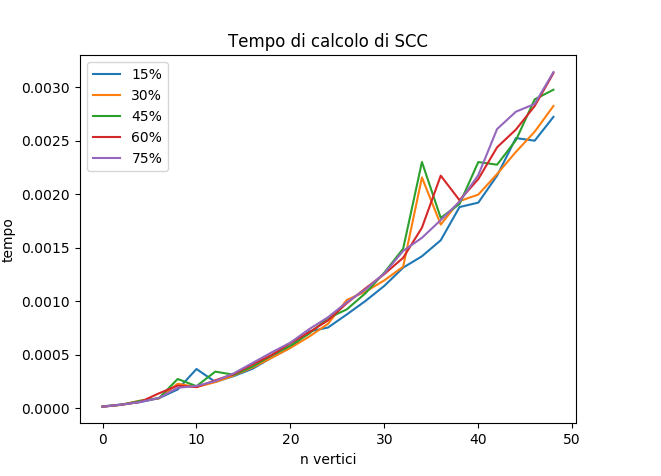
\includegraphics[scale=0.7]{tempo.png}

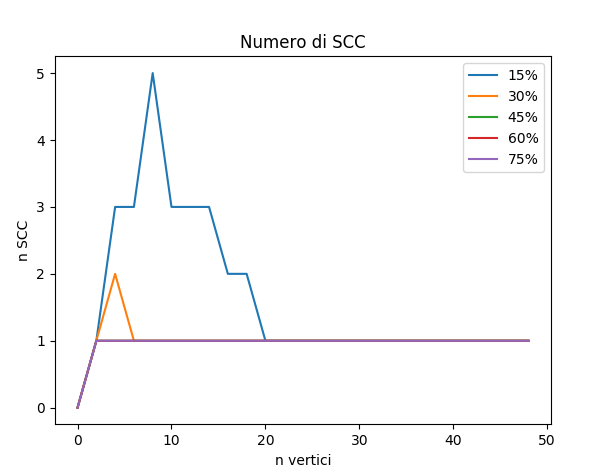
\includegraphics[scale=0.7]{alberi.png}

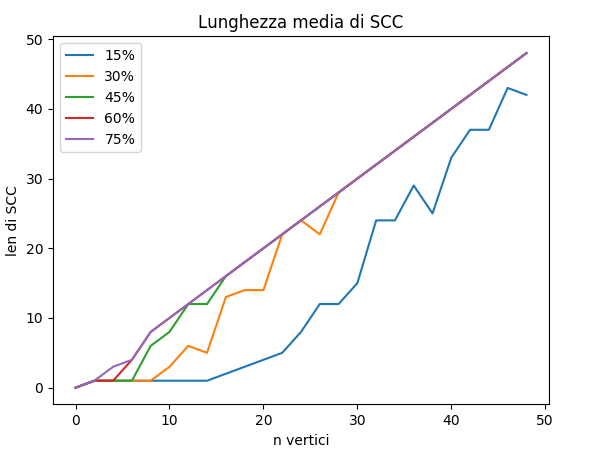
\includegraphics[scale=0.7]{nodi.png}


\end {document}